\begin{textblock}{38.0}(4,40)
\begin{block}{High Energy Physics (HEP)}
%\begin{center}
The quest to understand the fundamental building blocks of nature,
and their interactions, is one of the longest running and most
ambitious of human endeavors. Facilities such as the Large Hadron
Collider (LHC), where we do our research, represent a huge step
forward in our ability to answer these questions. The discovery of
the Higgs boson, the observation of exceedingly rare decays of B
mesons, and exclusion of countless theories beyond the Standard
Model (SM) of particle physics demonstrate that these experiments
deliver results. However, the most interesting fundamental physics
questions remain wide open, amongst them: What is the dark matter
which pervades the universe? Does space-time have additional
symmetries or extend beyond the 3 spatial dimensions we know? What
is the mechanism stabilizing the Higgs mass from enormous quantum
corrections? Are neutrinos, whose only SM interactions are weak,
their own anti-particles? Can the theories of gravity and quantum
mechanics be reconciled? Planned and running HEP experiments 
and facilities aim to answer these questions over the next 20 years. 
The computing and software challenges of these projects are formidable. 
The LHC experiments, for example, use nearly 0.5 Exabyte of
storage today in 170 computer centers in 42 countries. 
The upgrade to the High-Luminosity Large Hadron Collider (HL-LHC) will
increase the data volume
by more than a factor of 100, with significantly increased data and detector complexity. The resulting computing needs will outpace the expected improvements in computer performance (Moore's Law) by factors of between 3 and 30. 

\begin{figure}[tbph]
\centering
%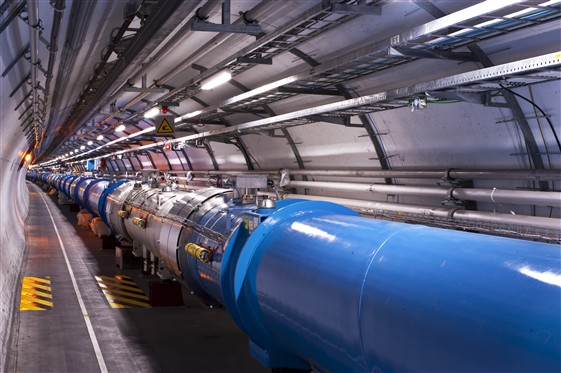
\includegraphics[width=0.48\textwidth]{images/0910152_02-A5-at-72-dpi.jpg}
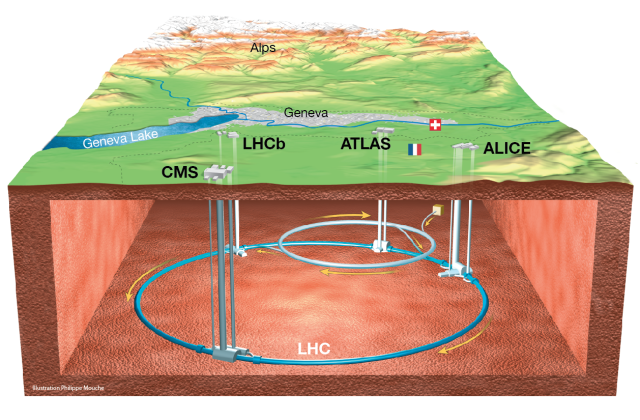
\includegraphics[width=0.41\textwidth]{images/CERN-LHC-cutaway-view-medium.png}
%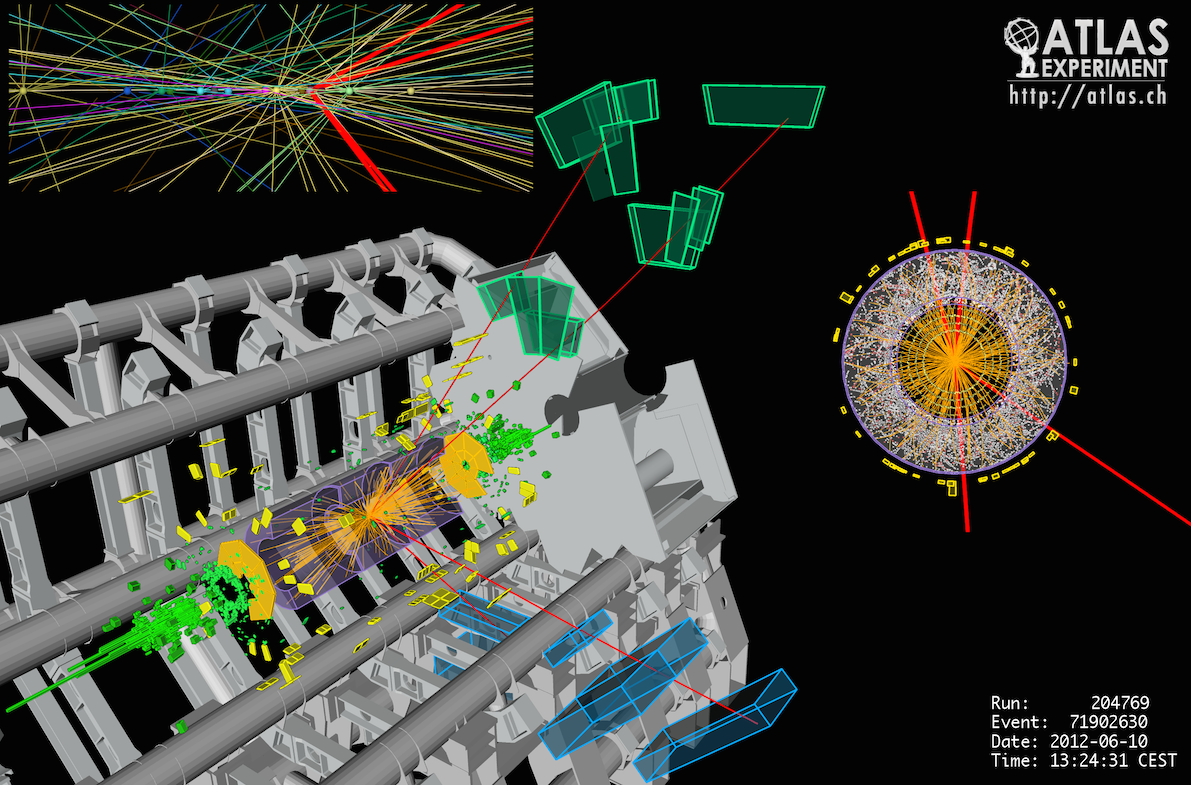
\includegraphics[width=0.41\textwidth]{images/run204769_evt71902630_VP1Base-half.png}
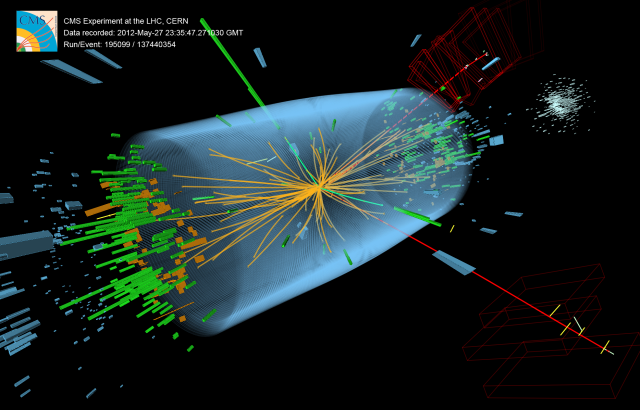
\includegraphics[width=0.42\textwidth]{images/eemm_run195099_evt137440354_ispy_3d-annotated-2.png}
%\begin{center}
%\end{center}
\end{figure}
{\small \copyright~2009-2016 CERN (License: CC-BY-SA-4.0)}
\end{block}
\end{textblock}




\begin{textblock}{38.0}(44,40)
\begin{block}{S2I2-HEP and the HEP Software Foundation}
Our S2I2-HEP strategic plan will describe how an NSF S2I2, and the
U.S.\ university community, could provide leadership and enable the
science of the HL-LHC era.  HEP experiments involve international
collaborations and a global software ecosystem, however, and the
activities of a possible S2I2 for HEP would need to fit into a
larger international context. To that end, we are also working with
the HEP Software Foundation (HSF) to develop on the same time scale
a ``Community White Paper'' (CWP) with a global roadmap for HEP
Software and Computing R\&D for the 2020s. The aim of the CWP is
to identify and prioritise the software research and development
investments required:

\begin{itemize}
\item to achieve improvements in software efficiency, scalability and performance and to make use of the advances in CPU, storage and network technologies
\item to enable new approaches to computing and software that could radically extend the physics reach of the detectors
\item to ensure the long term sustainability of the software through the lifetime of the HL-LHC
\end{itemize}

Achieving consensus in a large international community is a complex task. We are modeling the CWP process on that used for the HEP ``decadal survey'' (Snowmass) process and using a mix of dedicated general and topical workshops, solicitations for topical white papers contributions and outreach sessions at pre-existing HEP meetings. Most major HEP stakeholders (experiments, labs, institutions, software projects) are being engaged.
\end{block}
\end{textblock}

